\documentclass[a4paper]{article}

\usepackage{amsmath, blindtext, float, graphicx, hyperref}
\usepackage[textwidth=8in,textheight=10in]{geometry}% http://ctan.org/pkg/geometry
\graphicspath{ {./images/} }
\title{CS224N Assignment 4: Report}
\author{Author: \textbf{Shubham Gupta}\\
    Student Number: \textbf{A0225160U}
        }

\begin{document}
\maketitle
\section{NMT with RNN}
\subsection{1G}
\begin{itemize}
    \item Masking sentences is critical for attention to work.
    \item In both the encoder and the decoder, they help set the attention to zero for the padded tokens and non-zero for the actual tokens.
    \item In the decoder, the prevent the decoder from "peaking" into the tokens in the future. This helps ensure that the decoder focusses only on the information from the past.
    \item They also prevent the decoder from predicting the \textit{pad} padding tokens that are usually present in every training batch. These tokens are not useful during prediction, since the sentence predicted generally ends with a <EOS> token instead. 
\end{itemize}
\subsection{1H-1I}
\begin{figure}[H]
    \centering
    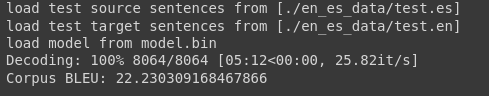
\includegraphics[width=0.3\textwidth]{bleu_score}
    \caption{Test Dataset BLEU Score: 22.230309168467866}
    \label{fig:bleu_score}
\end{figure}
\subsection{1J}
\begin{itemize}
    \item \textbf{Dot Product Attention}  
        \begin{itemize}
            \item Doesn't contain any learnable parameters. Simple to implement and less computationally expensive.
            \item No very expressive and only measures degree of alignment between encoder and decoder states.
        \end{itemize}
    \item \textbf{Multiplicative Attention} 
        \begin{itemize}
            \item More expressive and allows encoder and decoder to develop linearly dependent word vector representations.
            \item The final weight matrix doesn't have to be a square, hence embedding spaces can have different dimensions.
            \item More expensive compared to dot product variant. It simplifies the additive attention operation by computing
                $f_{att}(h_i, s_j) = h_i^TW_as_j$
            \item It does not work well as the number of dimensions increases.
        \end{itemize}
    \item \textbf{Additive Attention} 
        \begin{itemize}
            \item Decoder and encoder can develop independent embedding spaces.
            \item Mapping has more degrees of freedom and allows affine non-linear mapping between encoder and decoder space.
            \item Most computationally expensive operation as the number of operations grows by $O(N^2)$, where n in the sequence length.
            \item It works well for large dimensions of data.
        \end{itemize}
\end{itemize}
\section{Analyzing NMT Systems}
\subsection{A}
\begin{itemize}
    \item \textbf{I}  
    \begin{itemize}
        \item The word "favorite" is duplicate. The model output is correct in isolation i.e either "Here's another one of my favorites" or "Here's another favorite". 
        \item One way to resolve this error is to introduce attention over the translated sentence and use autoregressive-decoding to allow the model to focus on what has already been generated, thereby avoiding duplicates.
    \end{itemize}
    \item \textbf{II}  
    \begin{itemize}
        \item In this example, the model has performed a literal translation and missed the words from the spanish sentence "el autor para ninos, ms ledo" phrase which is a \textit{superlative} 
        \item We can solve this by adding additional exaples of superlatives to the corpus. This can be generated using tools such as nlpaug
    \end{itemize}
    \item \textbf{III}  
    \begin{itemize}
        \item Here, the translation sentence missed the word "Bolingbroke". This is likely because the word does not exist in the dictionary and does not have any occurence in the corpus. 
        \item One way to solve this would be to copy the word from the source sentence whenever the \textit{unk} token occurs. We can find the word using the attention weights. However, beware that this can also cause some false positives.
    \end{itemize}
    \item \textbf{IV}  
    \begin{itemize}
        \item In this example, the word "manzana" has two meanings: Apple and block. In the dataset, the meaning "Apple" occurs more frequently, which is probably the reason why it occurs in this prediction.
        \item We can solve this by including additional examples containing "manzana" with the context for "Block". We can also try to decode longer sequences to understand context better and 
    \end{itemize}
    \item \textbf{V} 
    \begin{itemize}
        \item Here, the word "teacher's" has been replaced by "women's". Similar to example I, the model output is correct in isolation. 
        \item This can be resolved by introducing attention over the translated sentence and allowing the model to focus on what has been generated.
    \end{itemize}
    \item \textbf{VI}  
    \begin{itemize}
        \item Here, we see that there are two different units of measurement used. In the source text, hectares is used, but in the groud truth, acres is used. We notice that the model has learnt the difference between units in US English and Spanish, but fails to produce the exact output since the literal translation does not perform numeric value conversion.
        \item We could use a post-prediction rule based system to detect different units and perform algorithmic translations.
    \end{itemize}
\end{itemize}
\subsection{B}
\begin{itemize}
    \item First Example:
    \begin{itemize}
        \item \textbf{Source Sentence}: Remi tiene 22 aos, es alto y muy guapo.
        \item \textbf{Reference Translation}:  Remi is 22,  tall and very handsome.
        \item \textbf{Machine Translation}: <unk> has 22 years old, it's high and very hot.
        \item Here, we notice that the model has no ability to determine the gender of OOV words(Remi). One way to fix this would be to introduce subword modelling such as Byte Pair Encoding, which will help break down OOV words.
        \item Furthermore, "alto" has been translated literally to "high" instead of the original word "tall". We can improve the performance of the model by adding longer sequences with varying contexts to the corpus.
    \end{itemize}
    \item Second Example:
    \begin{itemize}
        \item \textbf{Source Sentence}: Pienso que mi abuela naturalmente crea que todos sus nietos eran especiales.
        \item \textbf{Reference Translation}:  When I thought about my grandmother,  of course she would think all her grandkids were special.
        \item \textbf{Machine Translation}  I think my grandmother naturally believed that all their grandchildren were special.
        \item Here, we notice that the model incorrectly uses the plural "their" instead of the gender word "her". The gender is usually predicted wrong when the pronoun is far away.
        \item The gender for both grandfather and grandmother are wrong in a few examples in the predictions. Possible fixes for this problem including sub-word modelling to utilize the built in indicators of gender("father" and "mother") and training the model for a larger amount of time.
    \end{itemize}
\end{itemize}
\subsection{C}
\subsubsection{I}
\begin{equation}
\begin{split}
    C_1:  P_1 &= \frac{1}{5} (0 + 1 + 1 + 1 + 0) = \frac{3}{5} \\
    C_1:  P_2 &= \frac{1}{4} (0 + 1 + 1 + 0) = \frac{1}{2}\\
    r^* &= 4  \text{ and } c = 5 \\
    BP &= 7 \\
    BLEU &= 1 * ( \frac{1}{2} * \frac{3}{5} + \frac{1}{2} * \frac{1}{2}) = 0.55 \\
    \text{Similarly} \\
    C_2:  P_2 &= \frac{1}{5} (1 + 1 + 0 + 1 + 1) = \frac{4}{5} \\
    C_2:  P_2 &= \frac{1}{4} (1 + 0 + 0 + 1) = \frac{1}{2}\\
    r^* &= 4  \text{ and } c = 5 \\
    BP &= 7 \\
    BLEU &= 1 * ( \frac{1}{2} * \frac{4}{5} + \frac{1}{2} * \frac{1}{2}) = 0.65 \\
\end{split}
\end{equation}
\begin{itemize}
    \item Here, we notice that the 2nd translation is better. It is also the intuitive choice.
\end{itemize}
\subsubsection{II}
\begin{equation}
\begin{split}
    C_1:  P_1 &= \frac{1}{5} (0 + 1 + 1 + 1 + 0) = \frac{3}{5} \\
    C_1:  P_2 &= \frac{1}{4} (0 + 1 + 1 + 0) = \frac{1}{2}\\
    r^* &= 6  \text{ and } c = 5 \\
    BP &= 0.82 \\
    BLEU &= 0.82 * ( \frac{1}{2} * \frac{3}{5} + \frac{1}{2} * \frac{1}{2}) = 0.45 \\
    \text{Similarly} \\
    C_2:  P_2 &= \frac{1}{5} (1 + 1 + 0 + 0 + 0) = \frac{2}{5} \\
    C_2:  P_2 &= \frac{1}{4} (1 + 0 + 0 + 0) = \frac{1}{4}\\
    r^* &= 6  \text{ and } c = 5 \\
    BP &= 0.82 \\
    BLEU &= 0.82 * ( \frac{1}{2} * \frac{2}{5} + \frac{1}{2} * \frac{1}{4}) = 0.27 \\
\end{split}
\end{equation}
\begin{itemize}
    \item Here, we notice that according to the BLEU score, the first translation is better. This would not be the intuitive choice.
\end{itemize}
\subsubsection{III}
\begin{itemize}
    \item For task of sentence translation, each translated sentence has the chance of having some ambiguity about it. Hence, it's difficult to say that a sentence has only a single true translation.
    \item By providing multiple translations, we enable the NMT to learn about these various translations for the same input sentence. This will help the model generalize better and lead to an increase in the BLEU score.
    \item Having more than one reference translation will also allow the model to learn about how the translation changes based on the context of the sentence, which is important to create a good model.
\end{itemize}
\subsubsection{IV}
\begin{itemize}
    \item Advantages:
    \begin{itemize}
        \item It is fast and easy to calculate. It can be computed fast on computers, and helps us avoid using human translators to check the model output, which can be very expensive and time consuming.
        \item It's a universal metric. This makes it easy to compare our model to benchmarks on the same task.
    \end{itemize}
    \item Disadvantages:
    \begin{itemize}
        \item BLEU score does not consider meaning and the sentence structure. Since it only rewards n-grams that are exact matches, it will heavily penalize small gramatical errors which could be used to better understand the sentence by humans. Furthermore, since the sentence structure is not considered, words that are arbitarily written in the translated sentence will get the same score as the correct translation, as long as there are the same n-grams present.
        \item The BLEU scores on test-datasets are very specific, and their absolute value is not informative. Furthermore, BLEU does not map well to human judgements. Human translators can score very low on BLEU, possibly because of higher variability or the different word choices they use.
    \end{itemize}
\end{itemize}
\end{document}
